\documentclass[11pt,a4paper]{jsarticle}
	\usepackage{amsmath,amssymb}
	\usepackage{amsfonts}
	\usepackage{bm}
	\usepackage[dvipdfmx]{graphicx}
	\usepackage{ascmac}
	\usepackage{okumacro}
	\usepackage{titlesec}
	\usepackage{here}%画像を強制的に指定場所に置く[Here]を使える
	\usepackage{cases}%連立方程式など
	\usepackage{multicol}%複数段組
	\setlength{\textwidth}{\fullwidth}
	\setlength{\textheight}{39\baselineskip}
	\addtolength{\textheight}{\topskip}
	\setlength{\voffset}{-0.5in}
	\setlength{\headsep}{0.3in}
	%
	\makeatletter
	\def\section{\@startsection {section}{1}{\z@}{-2.5ex plus -1ex minus -.2ex}{2.5 ex plus .2ex}{\LARGE\bf}}
	\def\subsection{\@startsection {subsection}{1}{\z@}{-1.5ex plus -1ex minus -.2ex}{2.3 ex plus .2ex}{\Large\bf}}
	\def\subsubsection{\@startsection {subsubsection}{1}{\z@}{-2.5ex plus -1ex minus -.2ex}{.3 ex plus .2ex}{\large \bf}}
	\makeatother

	\makeatletter
	    \renewcommand{\theequation}{%
	    \thesection.\arabic{equation}}
	    \@addtoreset{equation}{section}
	  \makeatother


	\newcommand{\divergence}{\mathrm{div}\,}  %ダイバージェンス
	\newcommand{\grad}{\mathrm{grad}\,}  %グラディエント
	\newcommand{\rot}{\mathrm{rot}\,}  %ローテーション
	\newcommand{\pt}{\partial}  %パーシャル
	\newcommand{\df}{\overset{\mathrm{def}}{=}} %def
	\newcommand{\non}{\nonumber}  %\nonumber
	\newcommand{\dis}{\displaystyle}
	\newcommand{\f}[1]{\framebox[1cm]{\textgt{\small #1}}}
	\newcommand{\kine}{\frac{1}{2}mv^2} %運動エネルギー
	\newcommand{\sceq}{Schrödinger equation}
	\pagestyle{plain}
		%\markright{\footnotesize \sf 物理数学1A 第一回中間テスト(2017) 解答例 \ %左上のタイトル
		%{@sakuPonit}} %名前
\begin{document}

%% 表紙
\begin{center}
    \huge 平成30年度 物理学実験(二)\par
    \vspace{15mm}
    \Huge プランク定数 \par
    \vspace{60mm}
    \Large  実験日: 平成30年10月2日\par
    \vspace{15mm}
		\Large	実験者・筆者 1217054 佐久間寛伸\par
		\vspace{10mm}
		\Large	共同実験者 \par
						1217057 澤田大地 \par
						1217097 古谷優輝 \par
    \vspace{10mm}
  \end{center}
  \thispagestyle{empty}
  \clearpage
  \addtocounter{page}{-1}
  \newpage

%% 目次
\tableofcontents
  \newpage

%% 内容
\section{はじめに}
	\ 本報告書では書籍等からの引用をしている箇所がある.その被引用部で
	式番号が振られていた場合,本報告書内での式番号と重複・前後しないよう筆者がレポートの章立てに合うように適宜振り直しをした.
	そのため本報告書と引用元とでは式番号が異なることに留意されたい.

\section{目的}
	\ プランク定数測定器により,ハロゲン灯の光を分光し,振動数が知られているいくつかの単色光と
	Sb-Cs光電管とを用いて光電効果(photo-electric effect)の実験を行なう.それらの結果から,
	光が粒子性を示すことを理解し,
	さらにプランク定数(Planck constant)$h$を求める.

\section{原理}
	\subsection{プランク定数とエネルギー量子}
		\ そもそもプランク定数とは「量子力学的な現象を特徴づける普遍定数.
		ドイツの物理学者プランクが熱放射の研究のなかで1900年に発見した.」 \cite{planckconst01}物理定数である.
		ここでは『発見した』とあるが,
		「M.プランクは空洞放射の測定値を十分説明できる関係式(プランクの放射式)を見出したが,
		この式を導き出すには,振動数$\nu$の振動子のエネルギーの放出・吸収が連続的ではなく,
		$h \nu$を単位とする不連続な量の放出・吸収だけが許される,と仮定せざるをえなかった.
		ただし,$h$はプランク定数である.」 \cite{planckconstブリタニカ}
		のような,定数を『仮定』したという表現が適切と考える.
		\par また,『$h\nu$を単位とする不連続な量』をエネルギー量子(energy quantum)
		といい,これについては
		「$h \nu$をエネルギー量子という.エネルギー量子の考えは,
		エネルギーの連続性を根本的な足場にしている古典物理学の自然観と正面から対立し,
		量子論を生み出す第一歩となった.この功績により,1918年プランクにノーベル物理学賞が授与された.
		プランクのエネルギー量子という考えは,A.アインシュタインによって光量子という考えに発展した.」
		\cite{planckconstブリタニカ}
		とあるように光電効果,ひいてはそれ以降の量子論に繋がる重要な概念である.

	\subsection{光電効果}
		\ 光電効果については
		「金属の表面に光を照射すると電子が飛び出す.この現象を光電効果(特に外部光電効果)といい,
		飛び出した電子を光電子(photo-electron)と呼ぶ.アインシュタイン(A. Einstein)は,
		1905年にプランク(M. Planck)のエネルギー量子の考え方を発展させ,
		振動数$\nu$の光が伝播することは$hv$のエネルギーを持つ粒子が空間を
		飛んでいくことであると考えた.ここで$h$はプランク定数である.このような光の粒子を光子または光量子
		(photon)と名付けた.光電効果は,光子が金属中の電子と衝突してそれが持っているエネルギーを一度
		に全部電子に与え,その結果電子が金属の表面から外に飛び出す現象と解釈される.したがって,電子が金
		属表面を越えて外に出るために要する最小のエネルギーを$E$とすると,飛び出した光電子が持つことのでき
		る最大の運動エネルギーEは
			\begin{equation}
				E = h\nu - e\varphi \label{workfunc01}
			\end{equation}
		である.ここに$e$は電子の電荷の符号を変えたもので,素電荷と呼ばれる.
		また$\varphi$は仕事関数(work function)とよばれ,金属の種類によって決まる.
		\par 式(\ref{workfunc01})で$E=0$,つまり
			\begin{equation}
				\nu_0 = \frac{e \varphi}{h} \label{threshold frequency}
			\end{equation}
		を満たす振動数$\nu_0$を限界振動数という.
		限界振動数以下の振動数$\nu \leq \nu_0$の光は,それがどんなに強くても,
		その金属表面から電子を飛び出させることはできない.」
		\cite{物理学実験}
		とある.
		\par また,光電流については以下のように説明されている.「光電管(photon-tube)に振動数が$\nu$の単色光を入射すると,受光面である陰極から電子が飛び出すので,
		この陰極(受光面) と陽極を結ぶ外の回路に電流が流れる.
		この電流を光電流(photo-current) と呼ぶ.」
		\cite{物理学実験}
		\par さらに,光電効果を利用してプランク定数を求める方法については
		以下の通りである.
		「このとき,陽極側が負になるように電圧をかけ,
		その電圧を増加して行くと,光電流は減少する.
		この負電圧と光電流の関係を表す曲線を外挿して
		光電流がゼロに対応する負電圧をもとめる.
		このとき,光電子がどんな運動エネルギーを持っていても,全て陰極に押し返されている.
		したがって,この負電圧を$-V_0$とすると,
		$E=eV_0$であるから,式(\ref{workfunc01})は,
			\begin{equation}
				eV_0 = h\nu - e\varphi \label{workfunc02}
			\end{equation}
		となる.いくつかの振動数\nuについて同様な測定を行い,$\nu$と$eV_0$の関係を求めると,それは直線となり,その
		勾配からプランク定数$h$が得られる.知られている$h$の値は($6.626176 \pm 0.000036) \times 10^{-34}$J \cdot{\rm s}である.\\
		また,この直線を外挿して,用いた光電管の受光面を形成している金属の表面物質の仕事関数 $\varphi$ が得られる.」
		\cite{物理学実験}
		\par なお,仕事関数について
		「光が$h\nu$のエネルギーを持つ粒子であることから,単色光を指定する場合に波長や振動数のほか,光子エネ
		ルギー(photon energy)も使用される.単位としては,通常,エレクトロン·ボルト(eV)を用いる.1エレク
		トロン·ボルト= $e \times 1 $ジュールである.」
		\cite{物理学実験}
		とある.筆者は高校生時代に「仕事関数$W$の単位はJである.」と習ったが,
		「仕事関数は電子ボルトを普通は単位と」する\cite{planckconstブリタニカ}ことを
		明示的に記しておく.また,

\section{実験}
	\subsection{実験装置}
			\  本実験で用いたプランク定数測定器は島津理化製HA-30A(図\ref{fig1})であり,製造元によると
			「島津独自のホログラフィックグレーティングを用いたモノクロメータは,純度の高い単色光を取り出せます.」
			\cite{ha30a}とあるが,ホログラフィックグレーティング(ホログラフィック回折格子)とは,基板上のフォトレジスト(光に反応し物性を変える)を2本のレーザの光干渉により正弦波状に形成することで作成されるグレーティング(回折格子)である.
			\cite{ホログラフィックグレーティング}
			\cite{島津回折格子}
				\begin{figure}[H]
							\begin{center}
								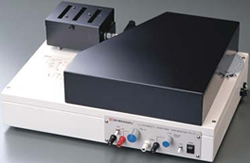
\includegraphics[width=80mm]{eqp01.jpg}
							\end{center}
							\caption{HA-30A \cite{ha30a}}
							\label{fig1}
						\end{figure} %HA-30A

			\par なお「島津独自の」という部分に関して,
			島津理化のホログラフィックグレーティングは独自技術によりブレーズ化が施されており
			ブレーズ化されていない回折格子に比べ
			特定の次数と波長に対して高い回折効率を示すという特長をもっている.
			ブレーズ化された,つまり溝の断面形状が鋸歯状である回折格子(ブレーズド回折格子)は,
			溝本数$N$,入射光の波長$\lambda_B$,取り出す回折光の次数$m$が決まっている場合,
			入射角を変化させ特定の入射角$\alpha$にすることで回折効率を高めることができる.
			この関係を満たすブレーズド回折格子の溝の傾きをブレーズ角$\theta_B$と呼び,
			入射光の波長$\lambda_B$をブレーズ波長と呼ぶ.$\lambda_B$は以下の式(\ref{ブレーズ波長})により求められる.
				\begin{equation}
					\lambda_B = \frac{2}{Nm} \sin{\theta_B} \cos{(\alpha - \theta_B)}
					\label{ブレーズ波長}
				\end{equation}
				\begin{figure}[H]
							\begin{center}
								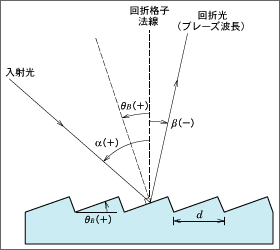
\includegraphics[width=70mm]{zu_05.png}
							\end{center}
							\caption{反射型回折格子 \cite{島津回折格子}}
							\label{ブレーズ波長}
						\end{figure} 

			この特性を用いて,本実験ではプランク定数測定器の"角度目盛盤"を操作し
			入射光に対するグレーティングの角度を変化させ,特定の単色光,つまり特定の波長を効率的に取り出している.
			\par 光電効果を定量的に計測するためには,短波長側から長波長へシャープに立ち上がる
			光源が必要である.この装置(HA-30A)では,ハロゲンランプを分光して得られるスペクトルを,
			スリットに通すことで連続的に単色光を得るようにしている.
				\begin{figure}
							\begin{center}
								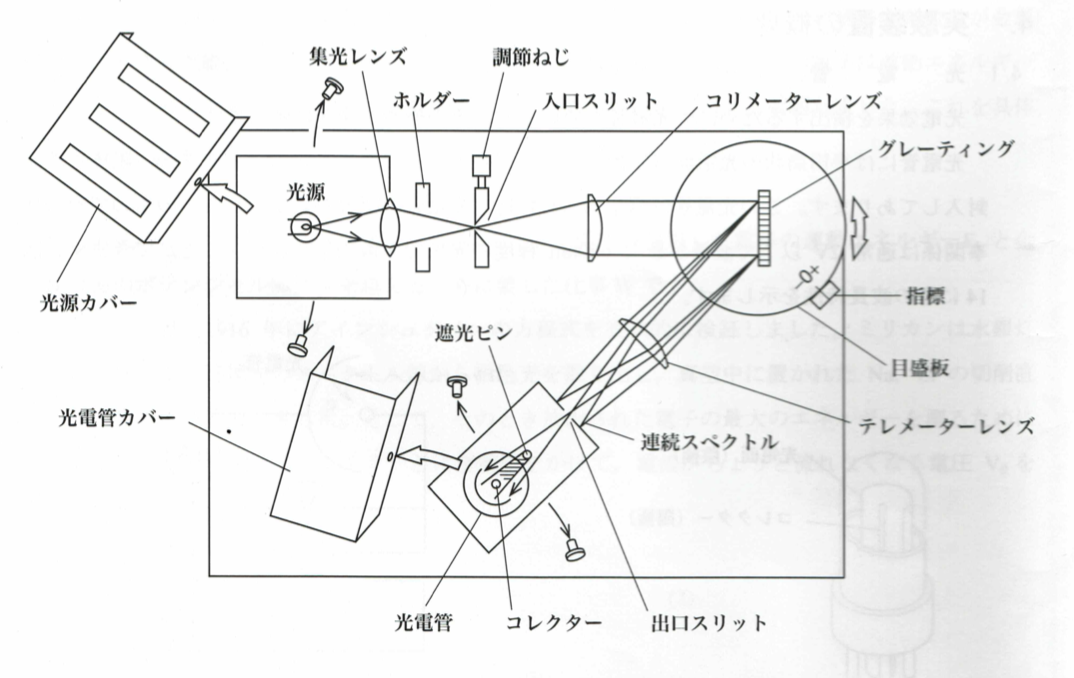
\includegraphics[width=100mm]{fig6.png}
							\end{center}
							\caption{分光器の構成 \cite{レタス}}
							\label{分光器の構成}
						\end{figure} 
				\begin{figure}
						\begin{center}
							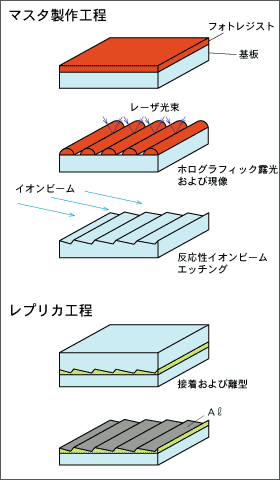
\includegraphics[width=70mm]{zu_01.png}
						\end{center}
						\caption{ブレーズド ホログラフィック グレーティの製作工程
						\cite{島津回折格子}}
						\label{ホログラフィックグレーティングの製造工程}
					\end{figure} 


			\par 図\ref{分光器の構成}は分光器の構成である.光源から出て,
			入口スリット上に集められた光は,コリメーターレンズで平行光になり,
			グレーティングで分光される.分光した光はテレメーターレンズで集光し,出口スリット位置に連続した入口スリットの像(すなわちスペクトル)
			として得られる.
			\par スペクトルのうち,出口スリットを通過した光は単色光として
			光電管に入射する.
			\par なお,入口スリットは調節ねじで間隔を変えられ,出口スリットは
			固定式になっている.図\ref{スペクトルと角度}は,角度目盛盤
			の数値を指標に合わせたとき,出口スリットを通過する中心波長を示す.角度0°から時計回りは(-),反時計回りは(+)の符号を付ける.
			\begin{figure}[H]
						\begin{center}
							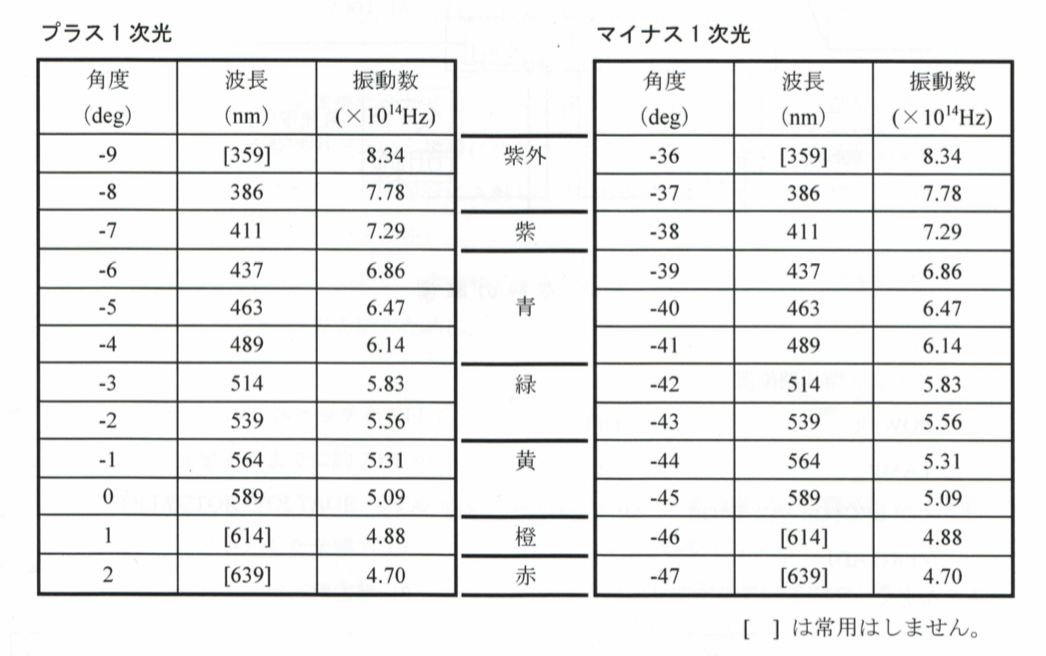
\includegraphics[width=120mm]{fig5.png}
						\end{center}
						\caption{スペクトルと角度 \cite{レタス}}
						\label{スペクトルと角度}
					\end{figure} 
	\subsection{実験手順}
		\subsubsection{準備}
			\begin{enumerate}
				\item 装置を机上にセットする.分光器カバー準備段階で外しておく.
				\begin{figure}
						\begin{center}
							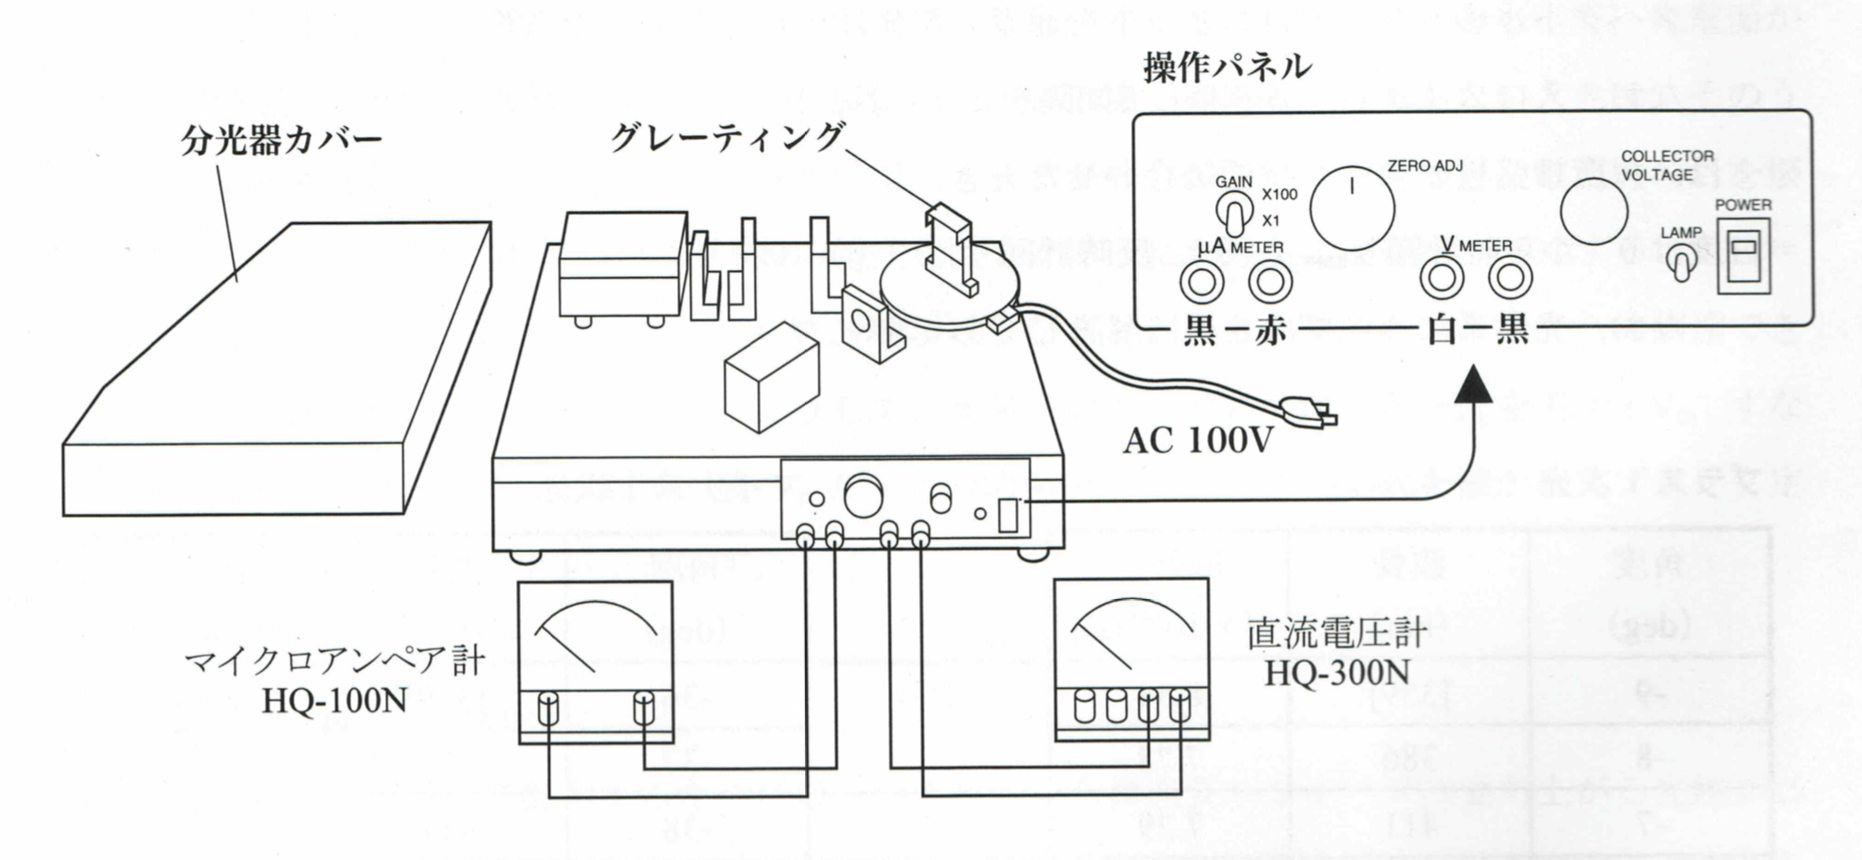
\includegraphics[width=100mm]{fig3.png}
						\end{center}
						\caption{実験の準備 \cite{レタス}}
						\label{実験の準備}
					\end{figure} 
				\item スイッチ類初期位置
					\begin{multicols}{2}
						POWER \\
						LAMP \\
						COLLECTOR VOLTAGE \\
						ZERO ADJ \\
						GAIN \\
						(OFF) \\
						(OFF) \\
						MIN(反時計いっぱい) \\
						中央 \\
						×1
					\end{multicols}
				\item メーターを図\ref{実験の準備}のように接続する.直流電圧計は白の端子がマイナス,
							黒の端子がプラスになるように接続する.
				\item 電源を接続する.以下,まず分光器の操作から説明する.
				\item POWERスイッチはOFFのままで,LAMPスイッチをONにする.(LAMPスイッチは電気回路のPOWERスイッチとは独立している.)
				\item 入口スリットは間隔が調節でき,つまみ1回転戻すと0.5mmの割合で広がる.スペクトルを目視する時は全開の状態から半回転ほど戻した状態にする.(図\ref{入口スリットと調節つまみ}) \\
				{\bf スリット調節つまみの使い方} \par
					\ スリットの開き加減は,スリットの光軸後方に紙片をかざし,点灯して透過光をみるとわかりやすい.
					\begin{enumerate}
						\item 調節つまみは上から見て時計回りが「開」方向である.
						\item つまみがやや重くなると,スリットが開き始める.1回転で0.5mm開く.つまみのマークで開き加減を把握することができる.
						\item 時計回りで行き止まったところがスリット幅約1mmである.それ以上は開かない.
							\begin{figure}[H]
									\begin{center}
										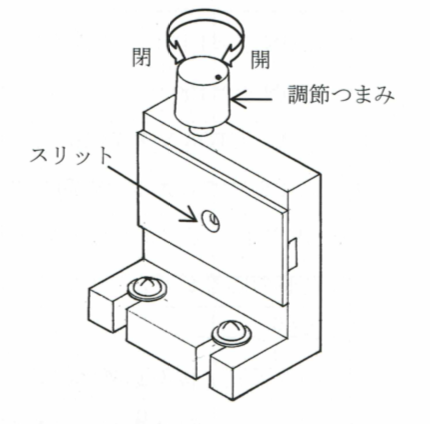
\includegraphics[width=50mm]{fig4.png}
									\end{center}
									\caption{入口スリットと調節つまみ \cite{レタス}}
									\label{入口スリットと調節つまみ}
								\end{figure} 
							\end{enumerate}
				\item 目盛盤の数値0°を標線に合わせる.光電管カバーの前面のスリット部分に連続スペクトルが見えることを確認する.標線に合わせる数値を,図\ref{スペクトルと角度}により設定すると,
				それぞれに対応する単色光が光電管に入射する.0位置では
				589nmなので,スペクトルの黄色の部分になる.
				\item 3箇所の穴にカバーの突起を一致させて分光器にカバーをかける.なお,外部からの迷光を防ぐために,分光器カバーをかけても装置のまわりはあまり明るくしないよう注意する.
				\item いったんLAMPスイッチをOFFにして,POWERをONにする.
				回路が安定するまでに約20分かかる.
				\item COLLECTOR VOLTAGEつまみをまわし,左いっぱいで直流電圧計の指示値が0V,右いっぱいにまわした状態で3V以上の電圧が出ることを確認する.
			\end{enumerate}
			逆電圧の可変には,精密級10回転ポテンショメータを使用しているので,操作は丁寧に行うよう注意する.
		\subsubsection{逆電圧/光電流のグラフ作成}
			\begin{enumerate}
				\item LAMPスイッチをOFFにする.
				\item 図\ref{スペクトルと角度}により,角度盤を-8°に正しく合わせる.386nm(紫外)光が光電管に入射できる.
				\item COLLECTOR VOLTAGEつまみを右に回し,3Vの逆電圧が光電管にかかった状態にしておく.
				\item LAMPスイッチをONにする,
				\item スリットをよく注意してみて,全開状態にする.さらにカバーの入射丸窓を紙片で塞ぐ.
				\item GAINを×1にし,直流増幅機バランス用のZERO ADJつまみを回してゼロ調節する.
				\item GAINを×100にしてもう一度ゼロ調節する.その後×1に戻す.
				\item COLLECTOR VOLTAGEを左いっぱいに回し切って,逆電圧を0Vにする.
				\item 紙片をはずし光量を調節する,GAINを×1にし,入口スリットをゆっくりと開き,逆電圧0Vにおいてマイクロアンペア計が,100µAを指すようにする.
				\item 逆電圧を3Vに戻す.このときµAメーターがほぼ0を指すことを確認する.
				\item GIAN×1でZERO ADJつまみを0調節した後,GAIN×100で注意深く0調節する.この調節の善し悪しが測定に大きく影響するので,1分ほど変化がないか確かめる.
				\item 逆電圧を3Vから徐々に小さくして行った時の光電流を\mu Aメーターで読む.
				\item 測定が終ったならばGIANを×1に戻す.
				\item 3.から12.までの操作を2˚ごと,すなわち
				-6˚(437nm),-4˚(489nm),-2˚(539nm),0˚(589nm)
				のそれぞれについて繰り返し逆電圧/光電流の値を取る.
				\item 光電流が流れ始める逆電圧を阻止電圧とするが,
				本報告書では0.01\mu Aで読み取る.
				\item 読み取った阻止電圧を縦軸に,対応する波長の振動数を横軸にプロットする.最小二乗法により回帰曲線を描き,その直線の傾きを求める.
			\end{enumerate}

\section{結果・考察}
	\subsection{結果}
		結果は図\ref{result1}の通りである.
		\begin{figure}[H]
				\begin{center}
					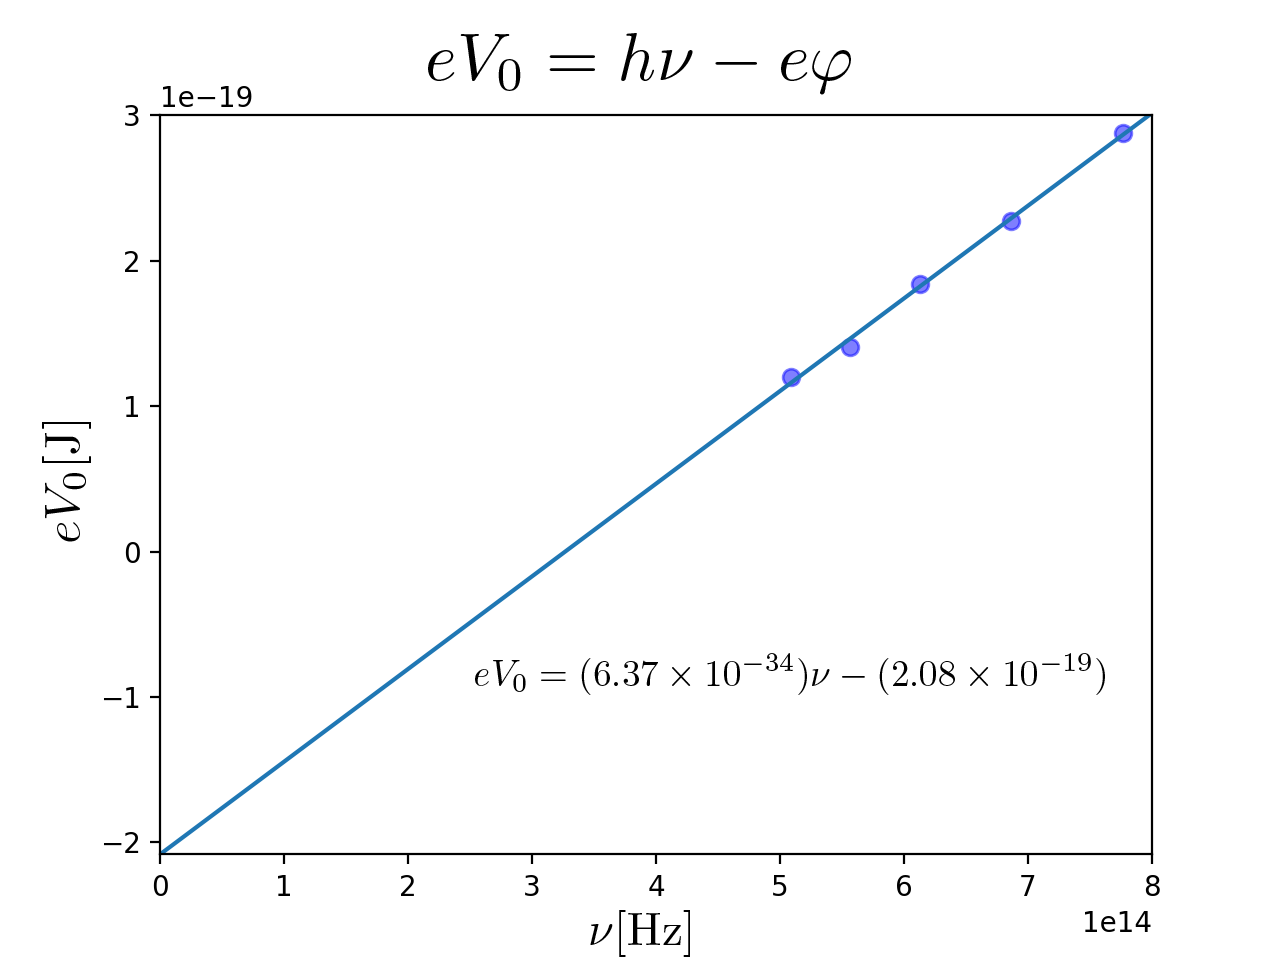
\includegraphics[width=120mm]{fig2.png}
				\end{center}
				\caption{単色光の周波数と阻止電圧の関係}
				\label{result1}
			\end{figure} %HA-30A
			回帰曲線からプランク定数$h$は
			\begin{equation}
				h = 6.37 \times 10^{-34} {\rm J \cdot s}
			\end{equation}
			であり,回帰曲線の切片$e\varphi=2.08 \times 10^{-19}$であることから仕事関数$\varphi$は,
			\begin{equation}
				\varphi = 1.3{\rm eV}
			\end{equation}
			である.
		\subsection{考察}
			知られているプランク定数は$6.626 \times 10^{-34} {\rm J \cdot s}$
			であるので\cite{物理学実験}実験値との相対誤差は
				\begin{equation}
					\frac{6.62 - 6.37}{6.62} \times 100 \simeq 3.8 \%
				\end{equation}
			である.そもそも本実験で使用したプランク定数測定器は10\%ほどの精度である\cite{ha30a}であるので
			,十分良い精度で実験できたと言えるだろう.
			また,使用したSb-Cs光電管について,Sb-Csの仕事関数$\varphi$は文献により様々な値
			が算出されている.(図\ref{Sb-Cs})
				\begin{figure}[H]
						\begin{center}
							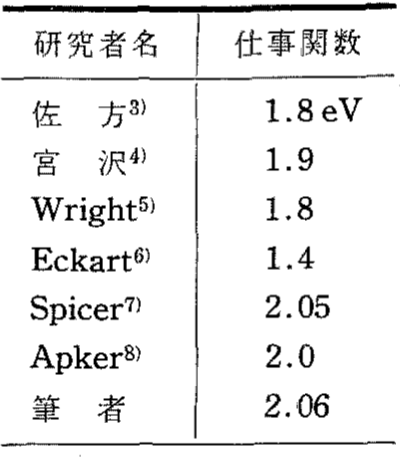
\includegraphics[width=50mm]{fig7.png}
						\end{center}
						\caption{Sb-Csの仕事関数 \cite{仕事関数}}
						\label{Sb-Cs}
					\end{figure} 
			しかし,図\ref{Sb-Cs}の値のうち,2eVを超えるものなどは可視光の長波長側で光電効果を起こさなくなる
			閾値に近く,今回の実験の結果と照らし合わせると必ずしも適合するとは言えない.したがって文献値とは乖離が見られるものの実験の失敗ではなく合金自体の違いであると考えられる.
			\par 全体的な誤差要因としてはゼロ調整の精度,電流計および電圧計の読み取りの精度,分光の精度などが考えられる.
			\par また,光の粒子性についてだが,本実験では減光の数値的な割合を記録していなかったので
			定量的な議論はできない.
			定性的には「50\%ほど減光したが阻止電圧はほとんど変わらなかった.光を単に波動であるとする
			ならば波のエネルギーは振幅の2乗に比例するので阻止電圧は減光前の4分の1になるはずであるので,光量子仮説を裏付ける結果が得られたと言える.」と述べることができる.



%% 参考文献
\begin{thebibliography}{9}
  \bibitem{planckconst01}江沢洋 『日本大百科全書(ニッポニカ)』 小学館
  \bibitem{planckconstブリタニカ}『ブリタニカ国際大百科事典 小項目事典』 ブリタニカ・ジャパン
  \bibitem{物理学実験}東京理科大学 理学部第一部 物理学教室 『物理学実験(二)』 (2018)
	\bibitem{ホログラフィックグレーティング}Palmer, Christopher, {\sl Diffraction Grating Handbook}, 6th edition, Newport Corporation (2005)
	\bibitem{島津回折格子}島津理化HP 製品情報 - 回折格子(グレーティング)の解説
	\bibitem{ha30a}島津理化HP 製品情報 - プランク定数測定器 HA-30A
	\bibitem{レタス}プランク定数測定器の取扱説明書
	 (https://letus.ed.tus.ac.jp/course/view.php?id=81223)
	\bibitem{仕事関数}萩野実 高橋正 和田正信『Sb(Mg)-Cs光 電面について』(1959)
	\end{thebibliography}

\end{document}
